\documentclass[12pt, letterpaper]{article}
\usepackage{polski}
\usepackage{xcolor}
\usepackage{amsmath}
\usepackage{graphicx}
\usepackage{hyperref}
\begin{document}
\definecolor{darkgreen}{RGB}{0,100,0} 
\renewcommand*\contentsname{Spis treści}
\begin{titlepage}
    \centering 
    
    \Huge 
    \textbf{Algorytmy Hashowania} 
    \vspace{1.5cm} %
    
    \Large 
    Autorzy: Kacper Kołaczkowski (72899), Jakub Stefaniak (73902)
    \vspace{1cm} 
    
    Data wykonania: 20 kwietnia 2024 
    \vspace{2cm} 
    
    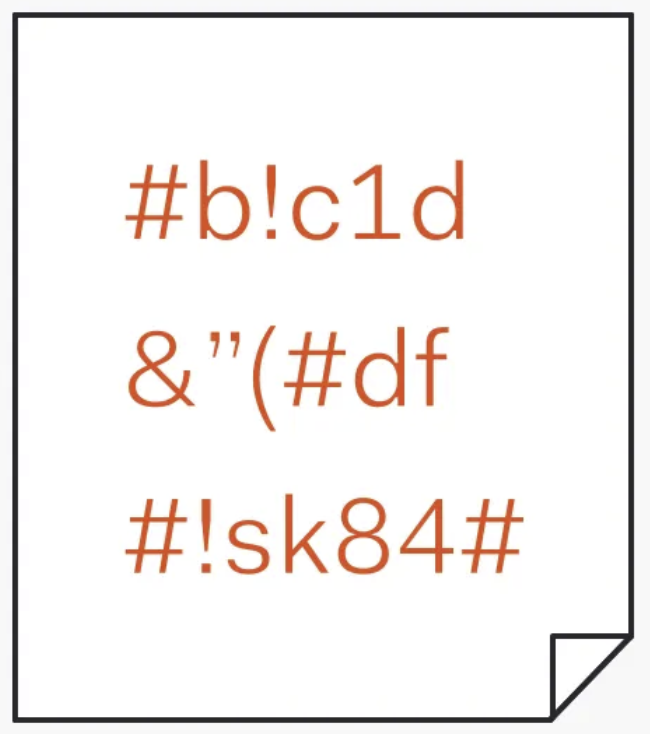
\includegraphics[width=0.5\textwidth]{hash.png} % Zdjęcie poniżej daty, centrowane
\end{titlepage}
\newpage
\tableofcontents
\newpage

\section{Hashowanie}
Proces generowania danych wyjściowych o stałym rozmiarze z danych wejściowych o zmiennym rozmiarze. Cały proces jest możliwy dzikęi zastosowaniu specjalnych wzorów matematycznych znanych pod nazwą tzw. funkcji mieszających (inaczej funkcji hashujących).

\section{Jak działa?}
Każda z istniejących funkcji skrótu na podstawie tych samych danych wejściowych generuje dane wyjściowe o innym od innych funkcji skrótu rozmiarów. To, co jednak łączy wszystkie algorytmy haszujące, to fakt iż, dana funkcja mieszająca na podstawie tego samego zestawu danych zawsze wygeneruje dane wyjściowe o tym samym rozmiarze. Dla przykładu algorytm hashujący SHA-256 po przepuszczeniu przez niego jakichkolwiek danych (czyt. danych wejściowych) wyprodukuje skrót o długości 256 bitów.

\section{Zapotrzebowanie}
\textbf{Bezpieczeństwo haseł:} Algorytmy haszujące są wykorzystywane do bezpiecznego przechowywania haseł użytkowników w systemach autoryzacyjnych.
\\
\\
\textbf{Integralność danych:} Haszowanie jest używane do sprawdzania integralności danych. Weryfikacja hasza pozwala szybko wykryć wszelkie zmiany w danych, nawet jeśli są one minimalne.
\\
\\
\textbf{Unikalność identyfikatorów:} W bazach danych, algorytmy haszujące są stosowane do generowania unikalnych identyfikatorów dla różnych rekordów.


\newpage
\section{BCrypt}
\textbf{BCrypt} to funkcja mieszania haseł i biblioteka szyfrowania szeroko wykorzystywana w rozwoju backendu w celu zapewnienia bezpiecznego przechowywania i weryfikacji haseł użytkowników. Pierwotnie zaprojektowany przez Nielsa Provosa i Davida Mazièresa dla systemu operacyjnego OpenBSD w 1999 roku, zyskał znaczną popularność w społeczności programistów dzięki solidnym funkcjom bezpieczeństwa i możliwościom adaptacji na różnych platformach.
\\
\\
Jest to algorytm oparty na funkcji haszującej, która konwertuje dowolną ilość danych wejściowych na wartość skrótu o stałej długości.
bCrypt wykorzystywany jest do zabezpieczenia haseł oraz innych poufnych informacji przed atakami hakerskimi. Dzięki zastosowaniu specjalnego algorytmu i tzw. "solenia" (dodanie losowo wygenerowanej wartości do hasła przed zahaszowaniem)  hasła, bCrypt jest w stanie skutecznie chronić przed atakami, które polegają na próbie odgadnięcia hasła poprzez przetestowanie wszystkich możliwych kombinacji. Bcrypt posiada maksymalną długość hasła do 72bitów.
\\
\\
Przykład prostego skryptu:

\textbf{Function bcrypt}
\begin{itemize}
   \item \textbf{Input:}
   \begin{itemize}
      \item \textit{cost}: Number (4..31) - $\log_{2}$(Iterations). np. 12 $\Rightarrow$ $2^{12}$ = 4,096 iteracji
      \item \textit{salt}: array of Bytes (16 bytes) - losowa sól
      \item \textit{password}: array of Bytes (1..72 bytes) - hasło zakodowane w UTF-8
   \end{itemize}
   \item \textbf{Output:}
   \begin{itemize}
      \item \textit{hash}: array of Bytes (24 bytes)
   \end{itemize}
\end{itemize}
\textcolor{darkgreen}{// Initialize Blowfish state with expensive key setup algorithm}
\\
\textcolor{darkgreen}{// P: array of 18 subkeys (UInt32[18])}
\\
\textcolor{darkgreen}{// S: Four substitution boxes (S-boxes), S0...S3. Each S-box is 1,024 bytes (UInt32[256])}
\\P, S $\leftarrow$ EksBlowfishSetup(password, salt, cost)
\\
\textcolor{darkgreen}{// Repeatedly encrypt the text "OrpheanBeholderScryDoubt" 64 times}
ctext $\leftarrow$ "OrpheanBeholderScryDoubt" \textcolor{darkgreen}{// 24 bytes $\Rightarrow$ three 64-bit blocks}
\textbf{repeat} (64)
\begin{itemize}
   \item ctext $\leftarrow$ EncryptECB(P, S, ctext) \textcolor{darkgreen}{// encrypt using standard Blowfish in ECB mode}
\end{itemize}
\textcolor{darkgreen}{//24-byte ctext is resulting password hash}\\
Przykład:
\\ masło $\rightarrow$ \$2a\$10\$.DAuQuU9CdP6SHdBzZ/rK.eXx9aS2fZSs8hxbEn0mXn0/7a1WmiN2
\\
\\
Każde zwiększenie współczynnika Work Factor o jeden zwiększa dwukrotnie czas obliczeń, gdy ten wynosi 11, obliczane są w 0.25 sekundy, natomiast gdy wynosi 14, są to już 2 sekundy.
Work Factor jest mechanizmem \textit{Key Stretchingu} bezpośrednio wbudowanym w sam algorytm funkcji.
\newpage
\section{MD5}
MD5 (ang. Message-Digest algorithm 5) algorytm, który z ciągu danych o dowolnej długości generuje 128-bitowy ciąg znaków.
Funkcja MD5 zdecydowanie nie powinna być używana w zastosowaniach wymagających odporności na kolizje, na przy5kład w podpisie cyfrowym.
Działa on następująco:
\begin{enumerate}
    \item Doklejenie do wiadomości wejściowej bitu o wartości 1
    \item Doklejenie takiej ilości zer, by ciąg składał się z 512-bitowych bloków i ostatniego niepełnego – 448-bitowego
    \item Doklejenie 64-bitowego licznika oznaczającego rozmiar wiadomości; w ten sposób otrzymywana wiadomość złożona jest z 512-bitowych fragmentów
    \item Ustawienie stanu początkowego na 0123456789abcdeffedcba9876543210
    \item Uruchomienie na każdym bloku funkcji zmieniającej stan
    \item Zwrócenie stanu po przetworzeniu ostatniego bloku jako obliczony skrót wiadomości
\end{enumerate}
\textbf{Przykład:}\\
\textit{komputer} → 71431b1e88117facdc7584c476e09452
\newpage
\section{SHA-1}
SHA-1 (ang. Secure Hash Algorithm) tworzy 160-bitowy skrót z wiadomości o maksymalnym rozmiarze \(2^{64}\) bitów i jest oparty na podobnych zasadach co MD5. Algorytm SHA-1 nie powinien być używany w nowych aplikacjach.

Skrypt:
Wartości początkowe:
\[ h0 := 0x67452301 \]
\[ h1 := 0xEFCDAB89 \]
\[ h2 := 0x98BADCFE \]
\[ h3 := 0x10325476 \]
\[ h4 := 0xC3D2E1F0 \]

Przetwarzanie wstępne:
\begin{itemize}
    \item dopisz '1' do wiadomości;
    \item dopisz \(k\) '0', gdzie \(0 \leq k < 512\) jest liczbą taką, że wynikowa długość wiadomości jest kongruentna do \(448 \mod 512\);
    \item dopisz długość wiadomości w bitach (przed wypełnieniem) jako 64-bitową liczbę całkowitą zakodowaną big endian.
\end{itemize}

Przetwarzaj wiadomość 512-bitowymi porcjami:
\begin{itemize}
    \item podziel wiadomość na 512-bitowe porcje;
    \item dla każdej porcji:
    \begin{itemize}
        \item podziel porcję na 16 32-bitowych słów kodowanych big-endian \(w(i)\), \(0 \leq i \leq 15\);
        \item rozszerz 16 32-bitowych słów do 80 32-bitowych słów:
        \[ \text{for } i \text{ from } 16 \text{ to } 79 \]
        \[ w(i) := (w(i-3) \oplus w(i-8) \oplus w(i-14) \oplus w(i-16)) <<< 1 \]
    \end{itemize}
\end{itemize}

Zainicjuj zmienne dla tej porcji:
\[ a := h0 \]
\[ b := h1 \]
\[ c := h2 \]
\[ d := h3 \]
\[ e := h4 \]

Główna pętla:
\begin{itemize}
    \item dla \(i\) od 0 do 79:
    \begin{itemize}
        \item if \(0 \leq i \leq 19\) then
        \[ f := (b \land c) \lor ((\lnot b) \land d) \]
        \[ k := 0x5A827999 \]
        \item else if \(20 \leq i \leq 39\) then
        \[ f := b \oplus c \oplus d \]
        \[ k := 0x6ED9EBA1 \]
        \item else if \(40 \leq i \leq 59\) then
        \[ f := (b \land c) \lor (b \land d) \lor (c \land d) \]
        \[ k := 0x8F1BBCDC \]
        \item else if \(60 \leq i \leq 79\) then
        \[ f := b \oplus c \oplus d \]
        \[ k := 0xCA62C1D6 \]
    \end{itemize}
\end{itemize}
\begin{align*}
    \text{temp} & := (a <<< 5) + f + e + k + w(i) \\
    e & := d \\
    d & := c \\
    c & := b <<< 30 \\
    b & := a \\
    a & := \text{temp}
\end{align*}

Dodaj skrót tej porcji do dotychczasowego wyniku:
\begin{align*}
    h0 & := h0 + a \\
    h1 & := h1 + b \\
    h2 & := h2 + c \\
    h3 & := h3 + d \\
    h4 & := h4 + e
\end{align*}

Wytwórz ostateczną wartość skrótu (zakodowaną big-endian):
\[ \text{skrót} = h0 \text{ dopisz } h1 \text{ dopisz } h2 \text{ dopisz } h3 \text{ dopisz } h4 \]
\newpage
\section{HMAC}
HMAC (ang. Hash Message Authentication Code) Standardowy kod MAC zapewnia ochronę integralności, ale może podlegać sfałszowaniu. Dla ochrony integralności i autentyczności w rozwiązaniach wymagających wysokiej wydajności stworzono zmodyfikowany algorytm MAC, w którym podczas każdej operacji dodawany jest tajny klucz:

\[ \text{HMAC}(K, m) = H((K \oplus opad) || H((K \oplus ipad) || m)) \]
\\
gdzie wartości \(opad\) i \(ipad\) są ustalonymi wartościami dopełniającymi, \(m\) jest tekstem podlegającym ochronie, a \(K\) jest tajnym kluczem. Tylko osoba znająca klucz \(K\) może zweryfikować autentyczność danych zabezpieczonych kodem HMAC. Implementacje HMAC są oparte na standardowych kryptograficznych funkcjach skrótu takich jak SHA-2, SHA-1 czy MD5. Kody HMAC są stosowane w szeregu protokołów sieciowych, np. w IPsec, gdzie klucze HMAC są niezależne od kluczy szyfrujących dane.

Przykład (z użyciem MD5):
\[ \text{komputer12} \rightarrow \text{11a1284ab371d7e20f9d0af92dc37759} \]
\newpage
\section{Argon2}
Argon2 jest nowoczesnym algorytmem szyfrowania jednostronnego. Jest on zalecany do szyfrowania haseł po tym jak wygrał konkurs Password Hashing Competition w Lipcu 2015.
\\
Algorytm został zaprojektowany w taki sposób, aby optymalnie wykorzystać dostępną pamięć oraz dostępne jednostki obliczeniowe, zapewniając jednocześnie ochronę przed atakami.
\\
W przeciwieństwie do Bcrypt, który mógł być parametryzowany tylko jednym czynnikiem - „koszt”, Argon2 jest parametryzowany przez trzy różne czynniki:
\begin{itemize}
    \item Koszt pamięci, który określa użycie pamięci przez algorytm.
    \item Koszt czasu, który określa czas wykonania algorytmu i liczbę iteracji.
    \item Współczynnik równoległości, który określa liczbę równoległych wątków.
\end{itemize}
Argon2 występuje w dwóch wariantach: Argon2i i Argon2d. Argon2i lepiej nadaje się do szyfrowania haseł i uzyskiwania kluczy na podstawie haseł, natomiast Argon2d jest szybszy i wysoce odporny na ataki polegające na łamaniu GPU.
\\
Dostępne są dwa główne warianty Argon2:

\begin{itemize}
    \item \textbf{Argon2i}: Skierowany do zastosowań, które wymagają wysokiej odporności na ataki typu side-channel, np. do przechowywania haseł i uzyskiwania kluczy na podstawie haseł.\\
    \item \textbf{Argon2d}: Skupia się na wysokiej wydajności i odporności na ataki przy użyciu GPU. Jest bardziej odpowiedni do obliczeń o dużej równoległości.
\end{itemize}
\newpage
\textbf{Podstawowy skrypt dla Argon2 wygląda tak:}

\begin{verbatim}
  Input:
    P (password to be hashed),
    S (salt),
    m (memory cost),
    t (time cost),
    p (parallelism),
  Output:
    H (resulting hash)
  
  1. Initialize memory blocks based on 'm'
  2. Initialize the first memory block with P and S
  3. For 't' iterations:
     a. Fill memory with a sequence of blocks derived from previous blocks, 
        depending on 'p'
  4. Return H as the hash of the final memory block
\end{verbatim}

To jest podstawowy zarys działania Argon2. W praktyce parametry 'm', 't', i 'p' mogą być dostosowane w zależności od wymagań bezpieczeństwa i wydajności.

\newpage
\section{Podsumowanie i wnioski}
W niniejszym tekście przedstawiliśmy przegląd algorytmów hashujących, które są szeroko stosowane w dziedzinie bezpieczeństwa komputerowego i weryfikacji integralności danych.
\\
\\
Przedstawiliśmy różne zastosowania algorytmów hashujących:
\begin{itemize}
    \item \textbf{Bezpieczeństwo haseł}: Algorytmy te są używane do bezpiecznego przechowywania haseł użytkowników w systemach autoryzacyjnych.
    \item \textbf{Integralność danych}: Hashowanie pozwala weryfikować, czy dane nie zostały zmienione.
    \item \textbf{Unikalność identyfikatorów}: Algorytmy hashujące są stosowane w bazach danych do generowania unikalnych identyfikatorów.
\end{itemize}
Omówiliśmy także kilka konkretnych algorytmów:

\begin{itemize}
    \item \textbf{BCrypt} to popularna funkcja mieszająca haseł, która oferuje solidne funkcje bezpieczeństwa dzięki zastosowaniu "solenia" i możliwości ustawienia kosztu (work factor).
    \item \textbf{MD5} to algorytm generujący 128-bitowe skróty, który jednak nie powinien być używany w zastosowaniach wymagających odporności na kolizje.
    \item \textbf{SHA-1} tworzy 160-bitowy skrót, ale również nie jest zalecany do nowych aplikacji ze względu na podatność na kolizje.
    \item \textbf{HMAC} to zmodyfikowany algorytm MAC, który dodaje tajny klucz w procesie hashowania, co zapewnia ochronę integralności i autentyczności.
\end{itemize}
Podsumowując, algorytmy hashujące mają szerokie zastosowanie w zabezpieczeniach komputerowych, ale ich wybór powinien być przemyślany ze względu na potencjalne podatności na ataki. Zaleca się używanie bardziej nowoczesnych i bezpiecznych algorytmów, takich jak BCrypt czy SHA-256, zwłaszcza w kontekście bezpieczeństwa haseł.
\newpage
\section{Referencje}
Podczas pisania tego artykułu korzystaliśmy z następujących źródeł:

\begin{enumerate}
    \item \href{https://www.czarnaowca.it/2020/09/haslo-w-aplikacji-jaki-algorytm-hash-wybrac/}{https://www.czarnaowca.it/2020/09/haslo-w-aplikacji-jaki-algorytm-hash-wybrac/}
    \item \href{https://sekurak.pl/jak-bezpiecznie-przechowywac-haslo-w-bazie-odpowiedz-zapewne-zaskoczy-wiekszosc-z-was/}{https://sekurak.pl/jak-bezpiecznie-przechowywac-haslo-w-bazie-odpowiedz-zapewne-zaskoczy-wiekszosc-z-was/}
    \item \href{https://ideaprogramowania.pl/szyfrowanie-za-pomoca-argon2/}{https://ideaprogramowania.pl/szyfrowanie-za-pomoca-argon2/}
    \item \href{https://appmaster.io/pl/glossary/bcrypt-2}{https://appmaster.io/pl/glossary/bcrypt-2}
    \item \href{https://pl.wikipedia.org/wiki/HMAC}{https://pl.wikipedia.org/wiki/HMAC}
    \item \href{https://academy.binance.com/pl/articles/what-is-hashing}{https://academy.binance.com/pl/articles/what-is-hashing}
    \item \href{https://pl.wikipedia.org/wiki/MD5}{https://pl.wikipedia.org/wiki/MD5}
\end{enumerate}

Te źródła dostarczyły informacje, które zostały wykorzystane w naszym artykule.

\end{document}